\section{Auswertung}
\label{sec:Auswertung}
%***********************************************Auswertung a*************************
\subsection{Charakteristik des untersuchten Halogen-Zählrohrs}
Zur Untersuchung der Charakteristik des Halogen-Zählrohrs wird die gemessene Anzahl an Impulsen pro Minute auf Impulse pro Sekunde umgerechnet und gegen die angelegte Spannung aufgetragen.


\begin{longtable}{ccc}
  \caption{Messdaten zur Untersuchung der Charakteristik des Zählrohrs.}\label{tab:atab}\\
\toprule
$U$/$\si{\volt}$ &$N$/$\si{\minute}$&$N_\mathrm{sec}$/$\si{\second}$ \\

\midrule
\endhead
\midrule
\endfoot
450  & 0  & 0.0\\
460  & 35050  & \num{584.17(41)} \\
470  & 35724  & \num{595.40(41)} \\
480  & 36480  & \num{608.00(41)} \\
490  & 36574  & \num{609.57(41)} \\
500  & 36961  & \num{616.02(40)} \\
510  & 37141  & \num{619.02(40)} \\
520  & 36881  & \num{614.68(40)} \\
530  & 37379  & \num{622.98(40)} \\
540  & 37176  & \num{619.60(40)} \\
550  & 37276  & \num{621.27(40)} \\
560  & 37621  & \num{627.02(40)} \\
570  & 37201  & \num{620.02(40)} \\
580  & 37326  & \num{622.10(40)} \\
590  & 37541  & \num{625.68(40)} \\
600  & 37594  & \num{626.57(40)} \\
610  & 37640  & \num{627.33(40)} \\
620  & 37334  & \num{622.23(40)} \\
630  & 37986  & \num{633.10(40)} \\
640  & 38002  & \num{633.37(40)} \\
650  & 38058  & \num{634.30(40)} \\
660  & 37629  & \num{627.15(40)} \\
670  & 37353  & \num{622.55(40)} \\
680  & 37637  & \num{627.28(40)} \\
690  & 37815  & \num{630.25(40)} \\
700  & 37743  & \num{629.05(40)} \\
710  & 37716  & \num{628.60(40)} \\
720  & 37938  & \num{632.30(40)} \\
730  & 38047  & \num{634.12(40)} \\
740  & 38104  & \num{635.07(40)} \\
750  & 37755  & \num{629.25(40)} \\
760  & 37662  & \num{627.70(40)} \\
770  & 37877  & \num{631.28(40)} \\
780  & 38182  & \num{636.37(40)} \\
790  & 38128  & \num{635.47(40)} \\
800  & 38142  & \num{635.70(40)} \\
810  & 38252  & \num{637.53(40)} \\
820  & 37984  & \num{633.07(40)} \\
830  & 38063  & \num{634.38(40)} \\
840  & 38422  & \num{640.37(40)} \\
850  & 38423  & \num{640.38(40)} \\
860  & 38492  & \num{641.53(39)} \\
870  & 38650  & \num{644.17(39)} \\
880  & 38624  & \num{643.73(39)} \\
890  & 38462  & \num{641.03(39)} \\
900  & 38285  & \num{638.08(40)} \\
\bottomrule
\end{longtable}


In Tabelle \ref{tab:atab} finden sich die gemessenen Datentupel aus angelegter Spannung $U$ und gezählten Impulsen $N$ pro Minute. Zudem werden die hieraus berechneten Impulse pro Sekunde $N_\mathrm{sec}$ und die Breite des zugehörigen Vertrauensintervall $\frac{\sqrt{N_\mathrm{sec}}}{N_\mathrm{sec}}$ angegeben.\\
In Abbildung \ref{fig:a} findet sich die Zählrohrcharakteristik.
Da der Bereich der Dauerentladung mit der vorliegenden Messapparatur nicht erreicht wurde, und die Anzahl der gemessenen Impulse zum Ende der Messung wieder leicht sinkt, wird ein Fehler im Versuch vermutet und als Arbeitsbereich des Zählrohrs das Intervall von $\SI{480}{\volt}$ bis $\SI{870}{\volt}$ angenommen.
Es ergibt sich somit eine Plateaulänge von $\Delta U_\mathrm{P}=\SI{390}{\volt}$.
Im Arbeitsbereich des Zählrohrs wird eine lineare Ausgleichsrechnung mit python/scipy \cite{scipy} durchgeführt.\\
Es ergeben sich die Parameter der Ausgleichgraden $y=m\cdot x+b$ zu:
\begin{align}
  m=  \SI{0.061(5)}{\volt\per\second} \text{,}\\
  b=  \SI{587(4)}{\per\second}\text{.}
\end{align}

Aus der Steigung der Ausgleichsgraden lässt sich die Steigung $P_\mathrm{S}$ im Plateaubereich ablesen zu:
\begin{equation*}
  P_\mathrm{S}=\frac{\SI{6.1(5)}{\percent}}{\SI{100}{\volt}} \text{ .}
\end{equation*}
\begin{figure}
  \centering
  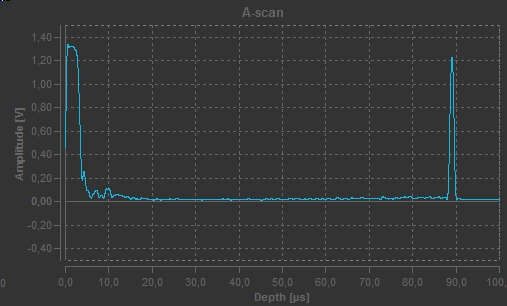
\includegraphics{Bilder/a.pdf}
  \caption{Zählrohrcharakteristik des Halogen-Zählrohrs samt markierter Plateaulänge und Ausgleichsgraden zur Bestimmung der Plateausteigung.}
  \label{fig:a}
\end{figure}
\FloatBarrier
%***********************************************

\subsection{Untersuchung von Nachentladungen}
Der Vergleich des Oszilloskopbilds bei einer geringen Betriebsspannung von etwa $\SI{450}{\volt}$ mit einer hohen Betriebsspannung von etwa $\SI{700}{\volt}$ zeigt, dass häufige und deutliche Nachentladungen lediglich für hohe Betriebsspannungen am Oszilloskopschirm sichtbar werden.
Nach Abbildung \ref{fig:nachladen} wird die Zeit zwischen dem ersten Impuls und den Nachentladungen abgelesen zu $\Delta t=\SI{175}{\micro\second}$.


\subsection{Bestimmung der Totzeit aus dem Oszilloskopbild}
Die Totzeit lässt sich nach Abbildung \ref{fig:nachladen} aus dem Oszilloskop ablesen.
In Tabelle \ref{tab:c} finden sich die bei verschiedenen Betriebsspannungen abgelesenen Totzeiten $T$, sowie die zugehörigen Erholungszeiten $T_\mathrm{E}$.
Da diese sich sehr willkürlich und nur ungenau bestimmen lassen, ist eine weitere Betrachtung der Erholungszeiten nicht sinnvoll.
\begin{table}
  \centering
  \caption{Messdaten zur Bestimmung der Totzeit aus dem Oszilloskopbild.}
  \label{tab:c}
\begin{tabular}{ccc}
  \toprule
$U$/$\si{\volt}$ & $T$/$\si{\micro\second}$ & $T_\mathrm{E}$/$\si{\micro\second}$ \\
\midrule
450  & 175  & 150  \\
500  & 175  & 100  \\
550  & 175  & 125  \\
600  & 175  & 150  \\
650  & 175  & 200  \\
\bottomrule
\end{tabular}
\end{table}
Eine Mittelung über alle Totzeiten ergibt eine mittlere Totzeit von $\overline{T}=\SI{175}{\micro\second}$.

\subsection{Bestimmung der Totzeit über die Zwei-Quellen-Methode}
\begin{table}
  \centering
  \caption{Messdaten zur Bestimmung der Totzeit über die Zwei-Quellen-Methode.}
  \label{tab:tot}
\begin{tabular}{ccc}
  \toprule
Quelle& $N$/$\si{\minute}$& $N$/$\si{\second}$ \\
\midrule
$N_1$ & 3499 & \num{58.3(1)} \\
$N_{1+2}$ & 49676 & \num{827.93(4)} \\
$N_{2}$ & 46298 & \num{771.63(4)} \\
\bottomrule
\end{tabular}
\end{table}
In Tabelle \ref{tab:tot} finden sich die gemessenen Impulsraten der Messung zur Bestimmung der Totzeit über die Zwei-Quellen-Methode.
Es wird erneut nach der Poisson-Verteilung ein Vertrauensintervall von $\pm\frac{\sqrt{N_i}}{N_i}$ angenommen.
Nach Formel \eqref{eqn:totzeit} ergibt sich die Totzeit zu:
\begin{equation}
  T=\SI{22.4(2)}{\micro\second}
\end{equation}

%Bild
%\begin{figure}
%  \centering
%  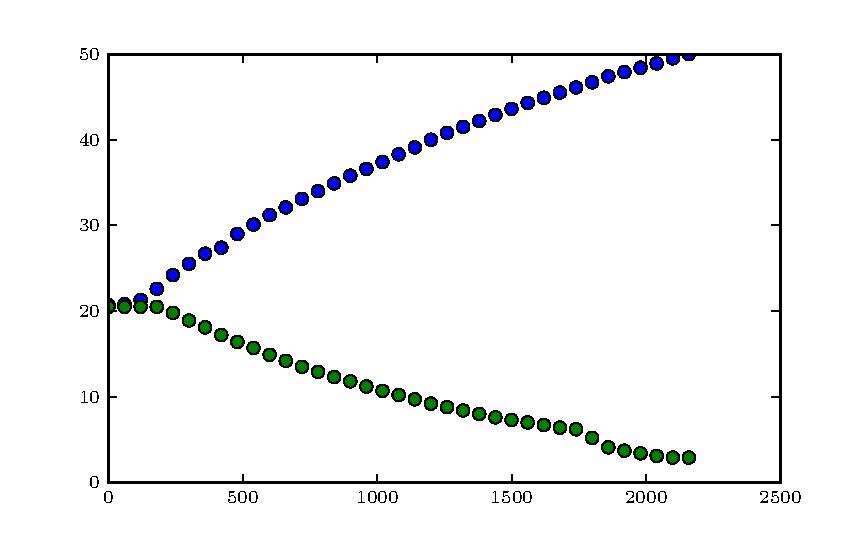
\includegraphics{plot.pdf}
%  \caption{Plot.}
%  \label{fig:plot}
%\end{figure}


%Tabelle
%\begin{table}
%	\centering
%	\caption{Table.}
%	\label{tab:table}
%	\begin{tabular}{ccc}
%		\toprule
%    column1&column2&column3\\
%		\midrule
%		220 & -391 & 659 \\
%		330 & -598 & 946 \\
%		525 & -1000 & 1660 \\
%		702 & -1337 & 2051 \\
%		930 & -1650 & 2450 \\
%		\bottomrule
%	\end{tabular}
%\end{table}
